% The entire content of this work (including the source code
% for TeX files and the generated PDF documents) by 
% Hongxiang Chen (nicknamed we.taper, or just Taper) is
% licensed under a 
% Creative Commons Attribution-NonCommercial-ShareAlike 4.0 
% International License (Link to the complete license text:
% http://creativecommons.org/licenses/by-nc-sa/4.0/).
\documentclass{article}

\usepackage{float}  % For H in figures
\usepackage{amsmath} % For math
\usepackage{amssymb}
\usepackage{bbm} % for numbers within mathbb
\usepackage{mathrsfs} % For \mathscr{ABC}
% Followings are for the special character: differential "d".
\newcommand*\diff{\mathop{}\!\mathrm{d}}
\newcommand*\Diff[1]{\mathop{}\!\mathrm{d^#1}}
\numberwithin{equation}{subsection} % have the enumeration go to the subsection level.
                                    % See:https://en.wikibooks.org/wiki/LaTeX/Advanced_Mathematics
\usepackage{graphicx}   % need for figures
\usepackage{cite} % need for bibligraphy.
\usepackage[unicode]{hyperref}  % make every cite a link
\usepackage{CJKutf8} % For Chinese characters
\usepackage{fancyref} % For easy adding figure,equation etc in reference. Use \fref or \Fref instead of \ref
\usepackage{braket} %http://tex.stackexchange.com/questions/214728/braket-notation-in-latex

% Following is for theorems etc environments
% http://tex.stackexchange.com/questions/45817/theorem-definition-lemma-problem-numbering && https://en.wikibooks.org/wiki/LaTeX/Theorems
\usepackage{amsthm}
\newtheorem{defi}{Definition}[section]
\newtheorem{thm}{Theorem}[section]
\newtheorem{lemma}{Lemma}[section]
\newtheorem{remark}{Remark}[section]
\newtheorem{prop}{Proposition}[section]
\newtheorem{coro}{Corollary}[section]
\theoremstyle{definition}
\newtheorem{ex}{Example}[section]

% A list of nomenclatures.
\usepackage{nomencl}
\makenomenclature

\usepackage[all]{xy} % For drawing diagrams with arrows
\title{Notes of Connecting Few-body and Many-body Pictures of Fractional Quantum Hall Physics}
\date{\today}
\author{Taper}


\begin{document}


\maketitle
\abstract{
    YouTube link\cite{utube-lecture}.
    Note that, although I have the video on hand, the lecturers are
    speaking somehow too fast and it would be too time-consuming to replay
    these lectures. So the content is..... quite unorgnised and bare.
    Therefore, this note could be viewed just as a collection of key
    words.
}
\tableofcontents
\section{Using Optical Emission to Study Competing Phase in the Second
Landau Level}
\label{sec:Using-Optical-Emission-to-Study-Competing-Phase-in-the-Second-Landau-Level}

By: 

Antonio Levy, Aron Pinczuk, Yuliya Kuznetsova (Columbia University),
Ursula Wurstbauer (Technische Uni. Munchen), Ken. W. West, Loren N.
Pfeiffer (Princeton), Michael J. Manfra, Geoff C. Gardner, John D. Watson
(Purdue University).

\paragraph{Overview} Second Landau Level displays
\begin{enumerate}
    \item FQHS
    \item Ordered phases (partially). RIQHE $ \overset{from}{\Leftarrow}$
        Electron stalids.
    \item Competition \& Coexistance

        Anisotropic FQHS arise from coorelation when anisotropic
        $\overset{from}{\Leftarrow}$ magneti field
\end{enumerate}
\paragraph{Advanage of Optial}
\begin{enumerate}
    \item Direct probes bulk
    \item Distinguish between charge and spin modes
\end{enumerate}
\paragraph{Sample} Omitted.
\paragraph{RRS}
$ $ % Go to the next line.

$ \xymatrix{
    \text{light}\ar[r] &
    \bullet\ar@/^/[r]^{\text{quasiparticle}}
                \ar@/_/@{<.}[r]_{\text{quasihole}} & 
    \bullet & \text{scattered photon}
}$

$\bullet$ Easy to probe Single Partical excitation and collective
excitation.

... (Skipped)

\section{Hyperspherical Adiabatic Approximation}
\label{sec:Hyperspherical-adiabatic-Approximation}

By: Rachel Wooten (Purdue University)

\paragraph{Outline}
\begin{enumerate}
    \item QHS
    \item Motivation
    \item Hyperspherical adiabatic approximation (\textbf{HAA})
    \item The role of degeneracy
    \item Hyperradial breathing mode
    \item Results and Discussion
\end{enumerate}

\paragraph{QHS}
\begin{table}[H]
    \caption{Two Schemes}
    \centering
    \begin{tabular}{|ccc|}
        \hline
        Conventional     & $\approx$ & Neutral Atom gass \\
        \hline
        2D Landau levels &           & 2D Rotation($\Omega$) \\
        $\omega_c$       &           & $\omega= 2\Omega$ \\
        \hline
    \end{tabular}
\end{table}

(Other schemes are also available, not treated).

\paragraph{Motivation}
\begin{itemize}
    \item QHS: prototype of \textit{Strongly correlated systems}
    \item Nature of few-body states
    \item insights from collectively coordinates
    \item use ... ?
\end{itemize}

\paragraph{Few body, adiabatic hypershperical approach\textbf{(AHA)}}

\begin{itemize}
    \item intrinsic collective coordinates
    \item length scale $R$ $\overset{\text{from}}{ \Leftarrow}$ geometry
    \item $E$ potential $ \Leftarrow$ length scale
    \item introduce Grand Angular momentum $K$ - quantum number
\end{itemize}

\paragraph{AHA background} Joe Macek, 1968 JPB.

\paragraph{Scheme} Sch-Ep $\overset{recast}{ \Rightarrow}$ relative
coordinates $ \overset{diagonalize}{ \Rightarrow}$ solve.

\paragraph{Hyperspherical Coordinates} $ $

$2N-2$ Jacobi coordinates $\Rightarrow$ $2N-3$ angular coordinates
$\Omega$ + 1 length coordinates Hyperradial $R$.
\begin{figure}[H]
    \centering
    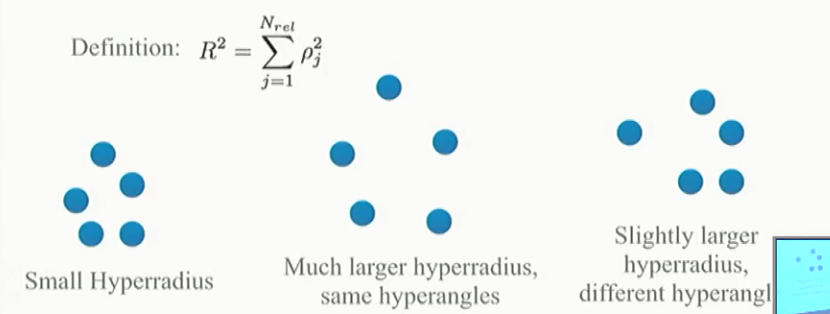
\includegraphics[width=0.8\linewidth]{pics/rachel-wooten-purdue.png}
\end{figure}

\paragraph{Hyperradius}
$$\rho = \left( \frac{\pi\mu\braket{R^2}}{N(N-1)} \right)$$
$$\mathscr{H}_\text{rel} = (R, \Omega, \cdots)
    +\text{Colomb} V(R)=\frac{1}{R}
    +\text{Polarized dipoles}V(R)=\frac{1}{R^3}
$$
\paragraph{AHA (Non-interacting case)} Omitted.
\paragraph{AHA (Interacting case)}$ $

Treat $R$ as an adiabatic parameter. 

Interaction $\overset{\text{introduct}}{\Rightarrow}$ degeneracies
\paragraph{Accuracy check} Omitted.
\paragraph{Exceptional degeneracy}

\section{? (Wick Haxton)}
\label{sec:Wick-Haxton}

(1995) Algebraic classification of general 4 fermion problem (Joe
Ginocchio) $\Rightarrow$ has FQHE implications

Jain \& Laughlin work (numerically succesful)

(No audio available for this lecture recording!, Skipped)

\section{Perspectives on the half-fill Landau Level}
\label{sec:Perspectives-on-the-half-fill-Landau-Level}

By B.I. Halperin, N. Copper, Chong Wong, Adey Stern.

\paragraph{Question}: What ahppens to half-filled Landau Level when there
is \textbf{NO} magnetic field.

\paragraph{Motivation}
\begin{itemize}
    \item New research on half-filled Landau level
    \item Describe system by "Dirac Fermion" is simpler, generated
        different theories $\Rightarrow$ doubt whether they are
        equivalent.
    \item Particle-hole symmetry in explicit in "Dirac Fermion", not
        explicit in HLR framwork.
\end{itemize}
\paragraph{Physical Setup} $ $

Half-filled Landau level: in a semiconductor.
$$ H_0 = \sum_i \frac{ |P_i - A(r_i)|^2}{2m} + V_2 \text{(interactions)}
$$
Units: $e=\hbar=1$.
\paragraph{PH Symmetry} $ $

\begin{itemize}
    \item $m\to 0$, e-e interactions are fixed -> exact PH symmetry
    \item For $v=1/2$, PHS requires that $\sigma_{xy}(\sigma)=(1/2) e^2/h$
\end{itemize}

\paragraph{HLR Approach}
(Halperin, Lee, Read. PRB 1993)

\begin{itemize}
    \item Singular gauge transformation $\Rightarrow$ Chern-Simons Gauge
        Field
    \item Transformed Hamiltonian will have fermion terms, interactions,
        gauge field (chern-simons interaction in it). Also the curl of a
        fact vector is constrained.
\end{itemize}
\paragraph{Antecednets}
\begin{itemize}
    \item Fractional Quantized Hall states by Jain; Lopez and Fradkin;
        others.
    \item Simultaneous work by Kalmeyer and Zhang had some features of
        HLR.
\end{itemize}

\paragraph{HLR Hypothesis}
\begin{itemize}
    \item Do mean field theory on this problem: the ground state and low
        energy properties of quantum hall system at $v=1/2$. And use
        perturbation theory and take into account of fluctuations in gauge
        field and Coulomb interactions
    \item ...
\end{itemize}
\paragraph{HLR consequences}
\begin{itemize}
    \item with $1/r$ interactions, the ground state is a "marginal fermi
        liquid". With mass diverges $log$ at fermi serface, eue to
        infrared divergence.
    \item assume interactions that fall off slower than $1/r$.
\end{itemize}
\paragraph{HLR-RPA predications}
\begin{itemize}
    \item ground state at $v=1/2$ should be compressible
    \item energy gaps, FQH states, occur at Jain fractions $v=p/(2p+2)$.
    \item relative sizes of energy gaps close to $1/2$
    \item transport in absence of impurities: DC hall conductance
    \item Longitudianl conductivity at finite $q,\omega\to 0$:
        $$\sigma_{xx}(q)=q/(8\pi k_f) $$
        in the presence impurities: formula holds for $q>l_{cf}$.
\end{itemize}

Related work: Kalmeyer \& Zhang.

\section{Anchor}
\label{sec:Anchor}

\begin{thebibliography}{1}
    \bibitem{utube-lecture}\url{https://www.youtube.com/playlist?list=PLCoSh1h28ieLIaD-HGi5aUQzunOTtxHTC}
\end{thebibliography}
\printnomenclature
\section{License}
The entire content of this work (including the source code
for TeX files and the generated PDF documents) by 
Hongxiang Chen (nicknamed we.taper, or just Taper) is
licensed under a 
\href{http://creativecommons.org/licenses/by-nc-sa/4.0/}{Creative 
Commons Attribution-NonCommercial-ShareAlike 4.0 International 
License}. Permissions beyond the scope of this 
license may be available at \url{mailto:we.taper[at]gmail[dot]com}.
\end{document}
